\documentclass{NSF}
\usepackage{cite}
\usepackage{soul}		% added for strike out
\usepackage{multirow} 	% added for centering text in the table
\usepackage{float}      % added for H to force figures to locations.
\usepackage{xfrac}      % math symbol extension
\usepackage{cmbright}
\usepackage{wrapfig}
\usepackage{xcolor}
\usepackage{listings}
\newcommand{\thedate}{\today}
\renewcommand{\thefigure}{\arabic{figure}}
\renewcommand{\thetable}{\Roman{table}}
\newcommand{\bl}[1]{\textcolor[rgb]{0.00,0.00,1.00}{#1}}
\newcommand{\gr}[1]{\textcolor[rgb]{0.00,0.50,0.00}{#1}}
\newcommand{\rd}[1]{\textcolor[rgb]{0.75,0.00,0.00}{\st{#1}}}
\newcommand{\tl}[1]{\textcolor[rgb]{0,0.6,0.60}{#1}}
\usepackage{titling}
\usepackage{graphicx}
\usepackage{hyperref}
\hypersetup{
	colorlinks=true,
	breaklinks=true,
	linkcolor=blue,    
	urlcolor=blue,
	citecolor=blue,}
\urlstyle{same}

\definecolor{codegreen}{rgb}{0,0.6,0}
\definecolor{codegray}{rgb}{0.5,0.5,0.5}
\definecolor{codepurple}{rgb}{0.58,0,0.82}
\definecolor{backcolour}{rgb}{0.95,0.95,0.95}

\lstdefinestyle{mystyle}{
	backgroundcolor=\color{backcolour},   
	commentstyle=\color{codegreen},
	keywordstyle=\color{magenta},
	numberstyle=\tiny\color{codegray},
	stringstyle=\color{codepurple},
	basicstyle=\ttfamily\footnotesize,
	breakatwhitespace=false,         
	breaklines=true,                 
	captionpos=b,                    
	keepspaces=true,                 
	numbers=left,                    
	numbersep=5pt,                  
	showspaces=false,                
	showstringspaces=false,
	showtabs=false,                  
	tabsize=2
}
\lstset{style=mystyle}

\graphicspath{{figures/}}

\begin{document}

% A. Cover Sheet
% A number of the boxes contained on the Cover Sheet are
% electronically pre-filled as part of the FastLane login process
% Complete the rest of your info there

\newsection{A}
\begin{titlepage}
	\centering
	
	% Include your institution's logo (if applicable)
	
\includegraphics[width=\textwidth]{AFRL-logo.png} % Replace "AFRL-logo.png" with the filename of your logo

	\vspace{2cm}
	
	\Huge{\textbf{Learning Mesh-Based Simulations for Predicting Weapon Effects}}
	
	
	\vspace{1cm}
	\begin{flushleft}
	
		\begin{large}
			\textbf{Program:} AFRL Scholars\\
			\vspace{1cm}
			\textbf{Mentor:} 
			\textit{\textbf{Dr. Alla Kammerdiner}, NRC/AFRL, Ph.D.Industrial and Systems Engineering}\\
			\vspace{1cm}
			\textbf{Researchers:}\\
			\begin{itemize}
				\item \textit{\textbf{Alexander B. Vereen}, Univeristy of South Carolina, B.S.E Mechanical Engineering} 
				\item \textit{\textbf{Caleb I. Fryer},Texas A\&M Univeristy, B.S Mechanical Engineering }
			\end{itemize}
		\end{large}

	\end{flushleft}
	
	\vfill
	
	\Large{\date{\today}}
	
\end{titlepage}

% B. Project Summary
\title{Learning Mesh-Based Simulations for Predicting Weapon Effects}
\newsection{B}
\section{Project Summary}
\subsection{Overview} 
This topic will address the fundamental challenges in real-time prediction of weapon effects (such as a tradeoff between precision and speed). Currently weaponeers rely on engineering models for lethality. These are low-fidelity models calibrated to a subset of munitions and environments. The resulting uncertainty often requires overallocation of munitions, which reduces the warfighter’s capabilities against adversaries. High fidelity simulations can reduce uncertainty but are too computationally intensive and time consuming to be used by weaponeers. The proposed research will utilize recent advances in Machine Learning (ML) methods to rapidly provide surrogate data to weaponeers (based on offline training on high fidelity simulation data). Specifically, selected scholars will learn how to apply MeshGraphNets to learn and predict mesh-based finite element simulations. Also, the scholars will compare MeshGraphNets with other ML methods. The scholars will advance their ability to code and perform numerical analysis. This work will provide the scholars valuable experience with state-of-the-art code for ML and high-fidelity simulations.\\


% C. Table of Contents 
% A Table of Contents is automatically generated for the proposal by FastLane


% D. Project Description
\newpage\newsection{D}
\section{Project Description}
\subsection{Introduction}
\subsection{Proposed Study}
Propose the usage:
the usage of mesh graph net as a replacement for simulation for analyzing operational deployment of ordinance

Purpose of the memo and study: Clearly state the reason for writing the memo and the objectives of the proposed study.\\
Background information: Provide a brief overview of the project or problem that the study aims to address.\\
Scope of the study: Outline the boundaries and limitations of the proposed study to set expectations for the readers.\\
Importance of the study: Explain why this study is crucial for the project or the organization.\\

\subsection{Current State of the Technology}
Existing technology overview: Provide an overview of the current technology, methodologies, or processes related to the subject matter.\\
Strengths and weaknesses: Identify the advantages and limitations of the current technology, highlighting areas that need improvement.\\
Industry trends: Briefly mention any emerging trends or advancements in the field that are relevant to the study.\\
Gap analysis: Identify the gaps between the existing technology and the desired goals to show the need for further investigation.\\

\subsection{Intended Impact}
Project objectives: Clearly state the intended outcomes and objectives of the proposed study.\\
Potential benefits: Explain the potential positive impacts the study could have on the project, organization, or industry.\\
Risk assessment: Address any potential risks or challenges that may arise during the study and how they will be mitigated.\\
Timeline and resources: Provide an overview of the estimated timeline and resources required to conduct the study.\\

% E. Background
\newpage\newsection{E}
\section{Background}
\subsection{Nueral Networks}
This is Caleb
\subsection{Graphs}

\subsection{Meshgraphnets}


% F. Environmental-config
\newpage\newsection{F}
\section{Environmental Configuration}
\subsection{Overview}

PyTorch and TensorFlow are two of the most popular deep learning frameworks used for building and training machine learning models. When setting up a development environment for working with these frameworks, having a Linux native environment or WSL2 (Windows Subsystem for Linux) can significantly ease the configuration process and subsequent usage with GPU acceleration, provided available Nivdia hardware. You can confirm your system hardware supports CUDA and cuDNN \href{https://developer.nvidia.com/cuda-gpus}{here}. Both PyTorch and TensorFlow offer GPU support, which allows for faster training times.

A Linux native environment or WSL2 is advantageous for configuring a machine learning environment in Python due to better package compatibility, efficient package managers, robust command-line tools, improved GPU support, enhanced reproducibility, and alignment with the machine learning community's practices.

\subsection{Windows Subsystem for Linux}
This section will breifly walk through how to install and enable WSL2 for your windows machine, documentation found \href{https://learn.microsoft.com/en-us/windows/wsl/install}{here}.
\begin{itemize}
	\item Launch PowerShell or Windows Command Prompt as an administrator by right-clicking and choosing "Run as administrator." then enable the usage of WSL and virtual enviroments by entering 
	\begin{lstlisting}[language=bash]
		Enable-WindowsOptionalFeature -Online -FeatureName Microsoft-Windows-Subsystem-Linux
		Enable-WindowsOptionalFeature -Online -FeatureName VirtualMachinePlatform\end{lstlisting}
	\item Next either download WSL from the window store or input the command
	 \begin{lstlisting}[language=bash]
	 	wsl --install\end{lstlisting} and then reboot your machine to complete the installation process.
	\item After the restart, open the Microsoft Store and search "Linux." You'll find various Linux distributions available. Choose the one that supports your intended version of CUDA refrenced below.
	\item After the installation is finished, launch the distribution from the Start menu or by searching for its name. The first time You run the Linux distribution, you will be prompted to set up a new Linux user and password.
	\item Configure your default linux distrobution to the installed distrobution using the powershell command \begin{lstlisting}[language=bash]
		wsl -s <DistributionName>\end{lstlisting}
\end{itemize}

You may now execute commands from Powershell to run in your install linux distrobution using the command "wsl" or "bash" to enter linux terminal.

\subsection{Linux Python Environment Management}

Before installing PyEnv, found \href{https://github.com/pyenv/pyenv}{here}, make sure you have the necessary dependencies in your WSL environment:
\begin{itemize}
	\item From bash within wsl run these commands
	\begin{lstlisting}[language=bash]
		sudo apt update
		sudo apt install -y git curl make build-essential libssl-dev zlib1g-dev libbz2-dev libreadline-dev libsqlite3-dev wget llvm libncurses5-dev xz-utils tk-dev libxml2-dev libxmlsec1-dev libffi-dev liblzma-dev \end{lstlisting}

	\item Next you may install PyEnv using curl
	\begin{lstlisting}[language=bash]
		curl https://pyenv.run | bash \end{lstlisting}
	
	\item Next you must add PyEnv to the Path environment variable using the following commands
	\begin{lstlisting}[language=bash]
		export PYENV_ROOT="$HOME/.pyenv"
		export PATH="$PYENV_ROOT/bin:$PATH"
		eval "$(pyenv init --path)"
		source ~/.bashrc \end{lstlisting}
	\item You may now install and manage multiple python enviroments separate from your Linux system Python environment using the follow commands:
	\begin{itemize}
		\item to list available Python versions
		\begin{lstlisting}[language=bash]
			pyenv install --list \end{lstlisting}
		\item to list install a Python version
		\begin{lstlisting}[language=bash]
			pyenv install <VERSION NUM> \end{lstlisting}
		\item to set the PyEnv virtual environment as the primary Python in enviroment 
		\begin{lstlisting}[language=bash]
			pyenv global <VERSION NUM> \end{lstlisting}
	\end{itemize}

\end{itemize}

\subsection{GPU configuration}

\begin{wrapfigure}{r}{0.5\textwidth}
	\vspace{-1.5cm}
	\begin{center}
		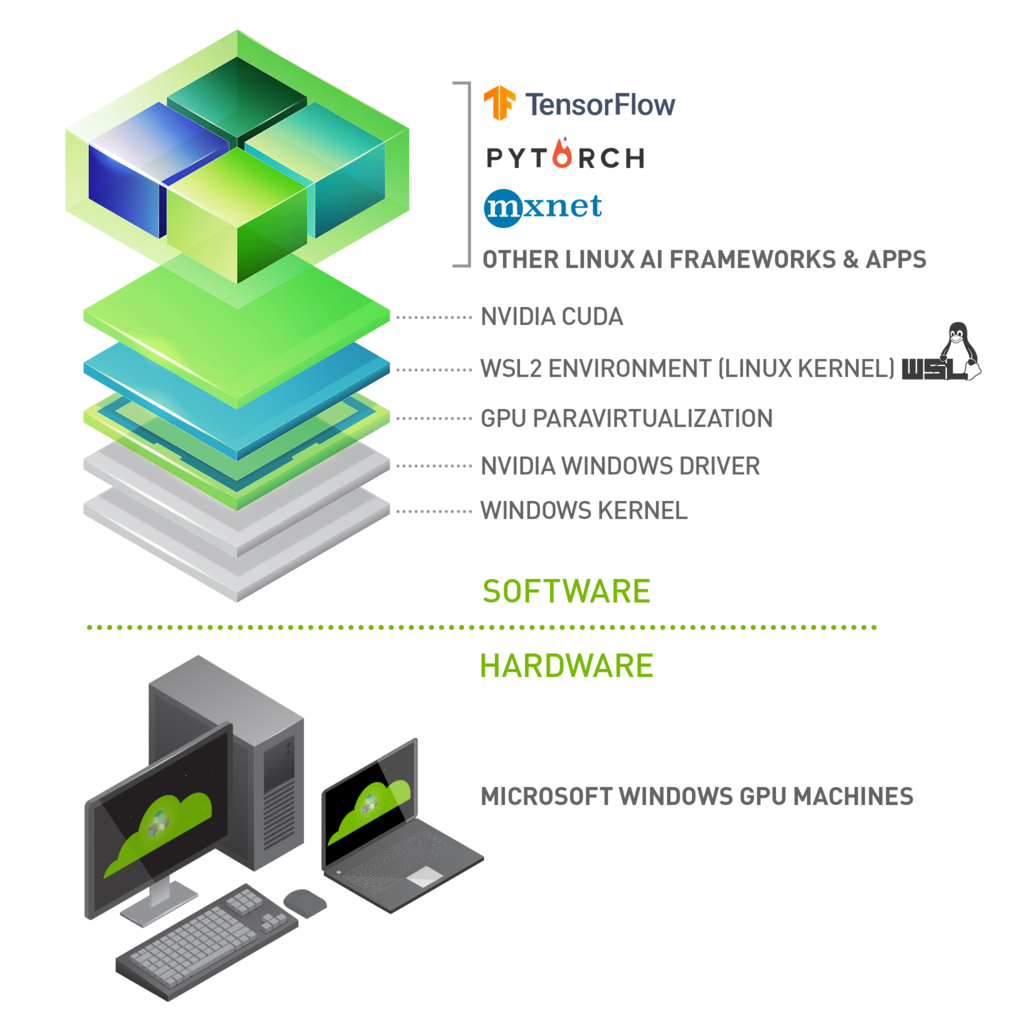
\includegraphics[width=.48\textwidth]{wsl-launch-upt-0625-rz.png}
	\end{center}
	\label{fig:arch}
\end{wrapfigure}

Now supported in WSL2, available for Window 10 and 11, and the Linux OS natively CUDA and cuDNN for running machine learning applications such a TensorFlow and PyTorch. Following the guidance available from Nvidia \href{https://docs.nvidia.com/cuda/wsl-user-guide/index.html}{here} the current release WSL 2 v1.2.5, released April 20, 2023, supported by Windows 10 and 11, uses a paravirtualizationShown in Fig.\ref{fig:arch} of the GPU architecture for the Linux subsystem to interact directly with the Window GPU driver. Whether using WSL2 as outlines in this guide or native linux installations the drivers can be found available from Nvidia \href{https://www.nvidia.com/Download/index.aspx?lang=en-us}{here} to enable the usage of CUDA and cuDNN for machine learning applications.

\pagebreak
\subsection{Environmental Configurations}
Detailed here is the environments used in this study, attached in the github :
\subsubsection{TensorFlow V1.X}
\begin{itemize}
	\item \textit{Python Version} == 3.6.x
	\item to install using pip
	\begin{lstlisting}[language=bash]
		pip install -r requirements.txt \end{lstlisting}
	\item to set the PyEnv virtual environment as the primary Python in enviroment 
	\begin{lstlisting}[language=bash]
		tensorflow-gpu==1.15
		dm-sonnet==1.36\end{lstlisting}
\end{itemize}
\subsubsection{PyTorch}
\begin{itemize}
	\item \textit{Python Version} == 3.10.x
	\item to install using pip
	\begin{lstlisting}[language=bash]
		pip install -r requirements.txt \end{lstlisting}
	\item to set the PyEnv virtual environment as the primary Python in enviroment 
	\begin{lstlisting}[language=bash]
		tensorflow-gpu>=1.15,<2
		dm-sonnet<2
		matplotlib
		absl-py
		numpy\end{lstlisting}
\end{itemize}




% G. Code-base
\newpage\newsection{G}
\section{Code base}
\subsection{Nueral Networks}

\subsection{Graphs}

\subsection{Meshgraphnets}

% H. Results
\newpage\newsection{H}
\section{Results}
\subsection{Metrics}

\subsection{test model: CFD}

\subsection{test model: Impact}


% I. Conclusion
\newpage\newsection{I}
\input{sections/conclusion}

% J. References Cited
\newpage\newsection{J}
\renewcommand\refname{References Cited}
\bibliography{references}
% I prefer to use the IEEE bibliography style. 
% That's  NOT required by the NSF guidelines. 
% Feel Free to use whatever style you prefer
\bibliographystyle{IEEEtran}

% K. Appendix
\newpage\newsection{K}
\input{sections/appendix}

\end{document}
